\documentclass{sig-alternate}
\usepackage[utf8]{inputenc}
\usepackage{hyperref}
\usepackage{comment}
\usepackage{array}
\usepackage{url}
\newcommand{\redcolor}[1]{\textcolor{red}{#1}}
\newcommand{\bluecolor}[1]{\textcolor{blue}{#1}}
\newcommand{\figref}[1]{Figure~\ref{#1}}
\newcommand{\secref}[1]{Section~\ref{#1}}
\newcommand{\appref}[1]{Appendix~\ref{#1}}
\newcommand{\tabref}[1]{Table~\ref{#1}}
\newcommand{\algoref}[1]{Algorithm~\ref{#1}}
\newcommand\Mark[1]{\textsuperscript#1}
\def\sharedaffiliation{\end{tabular}\newline\begin{tabular}{c}}


\def\iiitd{$^1$}
\def\imperial{$^2$}
\def\southampton{$^3$}
\def\ucla{$^4$}

% specialcell; see http://tex.stackexchange.com/a/19678
\newcommand{\specialcell}[2][c]{%
  \begin{tabular}[#1]{@{}c@{}}#2\end{tabular}}

\usepackage{xcolor,colortbl}
\usepackage{xfrac}

\title{NILMTK: An Open Source Toolkit for Non-intrusive Load Monitoring}

%\numberofauthors{1}

%\author{
%%	Nipun Batra\iiitd, 
%	Jack Kelly\imperial, 
%	Oliver Parson\southampton, 
%	Haimonti Dutta\iiitd,
%	William Knottenbelt\imperial,
%	Alex Rogers\southampton,
%	Amarjeet Singh\iiitd,
%	Mani B. Srivastava\ucla
%\sharedaffiliation
%  \begin{tabular}{cccc}
%    \affaddr{{\iiitd}Indraprastha Institute of Information Technology{\ }} & \affaddr{{\iiitd}Imperial College{\ }} & \affaddr{{\iiitd}University of Southampton{\ }} & \affaddr{{\ucla}University of California{\ }} \\
%    \affaddr{Delhi, India}                  &{London, UK} &{Southampton, UK} & \affaddr{Los Angeles, United States} \\
%\email{\{nipunb,manojg,amarjeet\}@iiitd.ac.in} & \email{\{jack.kelly,w.knottenbelt\}@imperial.ac.uk} & \email{\{op106,acr\}@ecs.soton.ac.uk}  & mbs@ucla.edu
%  \end{tabular}
%}

\author{Nipun Batra$^1$, Jack Kelly$^2$, Oliver Parson$^3$, Haimonti Dutta$^4$, William Knottenbelt$^2$,\\ Alex Rogers$^3$,Amarjeet Singh$^1$, Mani Srivastava$^5$\\ \\
\small$^1$Indraprastha Institute of Information Technology Delhi, India ~\{nipunb,~amarjeet\}@iiitd.ac.in\\
\small$^2$ Imperial College London ~\{jack.kelly,~wjk\}@imperial.ac.uk\\
\small$^3$ University of Southampton ~\{op106,~acr\}@ecs.soton.ac.uk\\
\small$^4$ CCLS Columbia ~\{haimonti@ccls.columbia.edu\}\\
\small$^5$ UCLA ~\{mbs@ucla.edu\}\\
}
%}
%T - number of time slices.

%t - a time slice.

%N - number of appliances.

%n - an appliance.

%K - number of states.

%k - an appliance state.

%\bar{y}^_t - measured aggregate power in time slice t.

%y^{(n)}_t - ground truth power of appliance n in time slice t.

%\hat{y}^{(n)}_t - estimated power of appliance n in time slice t.

%x(n)t - ground truth state of appliance n in time slice t.

%x^(n)t - estimated state of appliance n in time slice t.

\date{January 2014}

\begin{document}

\maketitle

%\begingroup
%\centering
%{\LARGE The Title \\[1.5em]
%\large First Author\Mark{1}, Second Author\Mark{2}, Third Author\Mark{1}, Fourth Author\Mark{2} and Fifth %Author\Mark{3}}\\[1em]
%\begin{tabular}{*{3}{>{\centering}p{.25\textwidth}}}
%\Mark{1}Department1 & \Mark{2}Department2 & \Mark{3}Department3 \tabularnewline
%School1 & School2 & School3 \tabularnewline
%\url{email1} & \url{email2} & \url{email3}
%\end{tabular}\par
%\endgroup


\begin{abstract}

\noindent
\textit{
Non-intrusive load monitoring, or energy disaggregation, aims to separate household energy consumption data collected from a single point of measurement into appliance-level consumption data. In recent years, the field has rapidly expanded due to increased interest as national deployments of smart meters have begun in many countries. However, empirically comparing disaggregation algorithms is currently virtually impossible, as a result of the different data sets used, the lack of reference implementations of these algorithms, and the variety of accuracy metrics employed. To address this challenge, we present the Non-intrusive Load Monitoring Toolkit~(NILMTK); an open source toolkit designed specifically to enable the comparison of energy disaggregation algorithms in a reproducible manner. Our toolkit includes parsers for a range of existing data sets, a standard output format for disaggregation algorithms, a set of statistics for describing data sets, two reference benchmark disaggregation algorithms, and a suite of accuracy metrics. We demonstrate that our toolkit makes it easier to enter into energy disaggregation research by simplifying the use of multiple data sets, while supporting the addition of new disaggregation algorithms, and also encouraging direct comparisons to be made between algorithms through common output formats and accuracy metrics. \bluecolor{This summary statement looks out of place. You may either make this claim earlier or just remove it from abstract.}In summary, this work is the first research to compare multiple disaggregation approaches across multiple publicly available data sets.}
\end{abstract}

\section{Introduction}

\noindent
Non-intrusive load monitoring (NILM), or energy disaggregation, aims to break down a household's aggregate electricity consumption into individual appliances~\cite{hart_1992}. The motivations for such a process are threefold. First, informing a household's occupants of how much energy each appliance consumes empowers them to take steps towards reducing their energy consumption~\cite{darby_2006}. Second, personalised feedback can be provided which quantifies the savings of certain appliance-specific advice, such as the financial savings when an old inefficient appliance is replaced by a new efficient appliance. Third, if the NILM system is able to determine the time of use of each appliance, a recommender system would be able to inform the household's occupants of the potential savings through deferring appliance use to a time of day when electricity is either cheaper or has a lower carbon footprint. %TO DISCUSS: do we also want to mention benefits of disaggregation for utility companies (they can do a better job of forecasting demand / managing the grid) and governments (easier to do large appliance usage surveys)?

Such benefits have drawn significant interest in the field since its inception 25 years ago. In recent years, the combination of smart meter meter deployments~\cite{CaliforniaPublicUtilitiesCommission2006,DepartmentofEnergy&ClimateChange2013} and reduced hardware costs of household electricity sensors has lead to a rapid expansion of the field. Such rapid growth over the past 5 years has been evidenced by the wealth of academic papers published, international meetings held \bluecolor{maybe add footnote URLs for these?}(e.g.\ NILM 2012, EPRI NILM 2013), startup companies founded (e.g. Bidgely, Neurio) and data sets released (e.g.\ REDD~\cite{redd}, BLUED~\cite{blued}, Smart*\cite{smart}).

However, three core obstacles currently prevent the direct comparison of state-of-the-art approaches, and as a result are limiting progress within the field. First, each contribution to date has only been evaluated on a single data set and consequently it is hard to assess the generality of any proposed approach. Furthermore, many researchers sub-sample data sets to select specific households, appliances and time periods, making experimental results more difficult to reproduce. Second, newly proposed approaches are rarely compared against the same benchmark algorithms, further increasing the difficulty in empirical comparisons of performance between different publications. Moreover, the lack of reference implementations of these state-of-the-art algorithms often leads to the reimplementation of such approaches. Third, each paper targets a different use case for NILM and therefore evaluates the accuracy of their proposed approach using a different set of performance metrics. As a result the numerical performance calculated by such metrics cannot be compared between any two papers. These three obstacles have led to the proposal of successive extensions to state-of-the-art algorithms, while a direct comparison between new and existing approaches has remained impossible.

Similar obstacles have arisen in other research fields and prompted the development of toolkits specifically designed to support research in that area. For example, PhysioToolkit offers access to over 50 databases of physiological data and provides software to support the processing and analysis of such data for the biomedical research community~\cite{physionet}. Similarly, CRAWDAD collects 89 data sets of wireless network data in addition to supporting software to aid the analysis of such data by the wireless network community~\cite{crawdad}. However, no such toolkit is available to the NILM community.

Against this background, we propose NILMTK\footnote{\url{github.com/nilmtk/nilmtk}}; an open source toolkit designed specifically to enable easy access to and comparative analysis of energy disaggregation algorithms across diverse data sets. NILMTK provides a complete pipeline from data sets to accuracy metrics, thereby lowering the entry barrier for researchers to plug in a new algorithm and compare its performance against the current state of the art. NILMTK has been:
\begin{itemize}
\item released as open source software in an effort to encourage researchers to contribute data sets, benchmark algorithms and accuracy metrics as they are proposed, with the goal of enabling a greater level of collaboration within the community. 
\item designed using a modular structure, therefore allowing researchers to reuse or replace individual components as required. 
\item written in Python with flat file input and output formats, in addition to high performance binary formats, ensuring compatibility with existing algorithms written in any language and designed for any platform.
\end{itemize}

\bluecolor{I think your contribution is NILMTK which has these sub-components. Each of them as a standalone probably does not deem fit as a contribution. Especially considering the space constraint you may chop this as well or restrict it to a few sentences. }Our contributions are summarised as follows:
\begin{itemize}
\item We propose NILMTK-DF (data format), the standard energy disaggregation data structure used by NILMTK.  NILMTK-DF is modelled loosely on the REDD data set format~\cite{redd}. Furthermore, we provide parsers from multiple existing data sets into our proposed NILMTK-DF format. In addition, we propose a single output format for the disaggregated data estimated by NILM algorithms.
\item We provide a set of statistical functions for detailed understanding of each data set.  We also provide a set of preprocessing functions for mitigating common challenges with NILM data sets.
\item We provide implementations of two benchmark disaggregation algorithms: first an approach based on combinatorial optimisation~\cite{hart_1992}, and second an approach based on the factorial hidden Markov model~\cite{REDD,kim_2011}. We demonstrate the ease by which NILMTK allows the comparison of these algorithms across a range of existing data sets, and present results of their performance.
\item We present a suite of accuracy metrics which are able to evaluate the performance of any disaggregation algorithm which produces an output compatible with NILMTK. This allows the performance of a disaggregation algorithm to be evaluated for a range of use cases.
\end{itemize}

The remainder of this paper is organised as \bluecolor{section 4 and 7}follows. In \secref{sec:related} we provide an overview of related work from the field of NILM and also other similar fields of research. In \secref{sec:nilmtk} we present NILMTK, and give a detailed description of its components. In \secref{evaluation} we demonstrate the empirical evaluations which are enabled by NILMTK, and provide analysis of existing data sets and accuracy metrics. Finally, in \secref{sec:conclusions} we conclude the paper and propose directions for future work.

\section{Background}
\label{sec:related}

\begin{table*}[]
  \centering
  \begin{tabular}{c c c c c c c c}
    \hline
    \bf Data set & \bf Institution & \bf Location & \bf Duration & \bf Number & \bf Appliance & \bf Aggregate\\
    \bf  & \bf  & \bf  & \bf per  & \bf of & \bf sample & \bf sample\\
    \bf  & \bf  & \bf  & \bf house & \bf houses & \bf frequency & \bf frequency\\
    \hline
    REDD (2011) & MIT & MA, USA & 3-19 days & 6 & 3 secs & 1 sec and 15 kHz\\
    BLUED (2012) & CMU & PA, USA & 8 days & 1 & N/A & N/A\\
    Smart* (2012) & UMass & MA, USA & 3 months & 1 & 1 sec & 1 sec\\
    Tracebase (2012) & Darmstadt & Germany & N/A & N/A & 1-10 second & N/A\\
    Sample (2013) & Pecan Street & TX, USA & 7 days & 10 & 1 min & N/A\\
    HES (2013) & DECC, DEFRA & UK & 1 or 12 months & 251 & 2 or 10 minute
    & 2 or 10 minute\\
    AMPds (2013) & Simon Fraser U. & BC, Canada & 1 year & 1 & 1 min & Yes\\
    iAWE (2013) & IIIT Delhi & Delhi, India & 73 days & 1 & 1 sec & 1 sec\\
    UKPD (2014) & Imperial College & London, UK & 3-14 months & 4 & 6 secs & 1-6 secs or 16 kHz \\
    \hline
  \end{tabular}
  \caption{Comparison of household energy data sets.\bluecolor{table going out of columns}}
  \label{table:datasets}
\end{table*}

\noindent
The field of non-intrusive load monitoring was founded over 20 years ago when Hart proposed the first algorithm for disaggregation of household energy usage~\cite{hart_1992}. Since then, many studies have shown the benefits of disaggregated data to both household occupants leading to financial savings, and also to utility providers providing demand response management~\cite{zeifman_2011,armel_2013}. However, majority of research had been evaluated using either lab-based or simulated data and hence the performance of disaggregation algorithms in real households has remained unknown. More recently, national deployments of smart meters have prompted a renewed interest in energy disaggregation. As a result a number of data sets, collected specifically for energy disaggregation have been released. We now discuss some of the publicly available data sets currently available an overview of which is presented in \tabref{table:datasets}.

In 2011, the Reference Energy Disaggregation Dataset (REDD)~\cite{redd} was the first publicly available data set, collected specifically to aid NILM research.. The data set contains both aggregate and sub-metered power data from 6 homes, and has since become the most popular data set for evaluating energy disaggregation algorithms. In 2012, the Building-Level fUlly-labeled dataset for Electricity Disaggregation (BLUED)~\cite{blued} was released containing data from a single household. However, the data set does not include sub-metered power data, and instead events triggered by appliance state change were recorded. \bluecolor{unclear what is the difference between inferring appliance activity and disaggregation of appliance.}As a result, it is only possible to evaluate how well appliance activity can be inferred, rather than the disaggregation of appliance energy consumption. More recently, the SMART*~\cite{smart} data set was released, which contains household aggregate power data from 3 homes, while sub-metered appliance power data was only collected from a single household.

In 2013 the Pecan Street sample data set was released~\cite{pecan}, which contains both aggregate and sub-metered data from 10 households. Later, the Household Energy Study data\bluecolor{needs a citation} set was released, which contains data from 251 households although only sub-metered \bluecolor{somewhere you use sub-metered power data (for REDD and BLUED) and somewhere sub-metered appliance data. Be consistent. I also feel that sub-metered is not the appropriate term. A suggestion - You may use separately-monitored }appliance data was collected. The Almanac of Minutely Power dataset (AMPds)~\cite{ampds} was also released that year containing both aggregate and sub-metered data from a single household. Subsequently, the Indian data for Ambient Water and Electricity Sensing (iAWE)~\cite{iawe} was released, which contains both aggregate and sub-metered electricity data from a single home. Most recently, the UK Power Dataset (UKPD)~\cite{ukpd} was released which contains data from four households using both aggregate meters and individual appliance sub-meters. Unfortunately, subtle differences in the aims of each data set have lead to completely different data formats being used.As a result a time-consuming engineering barrier exists when using the data sets, each of which are in different formats. This has resulted in publications using only a single data set to evaluate a given approach, and consequently the generality of results are rarely investigated. Having described the data sets that are currently available, we now discuss recent publications which have used such data sets for the evaluation of disaggregation algorithms.

%\bluecolor{you may summarize the literature using different datasets and their differences in a table if you need some more space}
\bluecolor{delete from REDD to .The}The REDD data set has been used to compare the performance of many disaggregation algorithms since its publication in 2011. The data set was proposed along with a performance result of a benchmark disaggregation algorithm using 10 second data across 5 of the 6 households~\cite{redd}. Kolter and Jaakkola later proposed an extension to the benchmark algorithm~\cite{kolter_2012}; however, the extension was only evaluated using features extracted from 14~kHz data from a single home from the data set, and therefore the performance results are not directly comparable. Later, Zeifman~\cite{zeifman_2012} and Johnson and Willsky~\cite{johnson_2013} evaluated various approaches using the same data set, although both selected a different subset of appliances and calculated an artificial household aggregate from these appliances, therefore simplifying the disaggregation problem and preventing a numerical comparison with other publications. Subsequently, Parson et al.~\cite{parson_2012} and Rahayu et al.~\cite{rahayu_2012} both proposed new approaches, although each were evaluated using a different set of 4 houses from the REDD data set, again preventing a numerical comparison between publications. Last, Batra et al.~\cite{batra_2013} evaluated their approach on the REDD data set using a different household to Kolter and Jaakkola. As a result, it has not been possible to deduce from literature whether one approach is preferable to another from the literature.

\bluecolor{delete and only write Similarly, BLUED was introduced}In addition to REDD, other data sets have been used to evaluate the performance of NILM algorithms. For example, BLUED was introduced along with a benchmark algorithm~\cite{blued}, but has since only been used by one other publication~\cite{anderson_2012}. Similarly, AMPds and iAWE have only been used to evaluate disaggregation algorithms proposed by the data set authors~\cite{ampds,iawe}. Clearly, the variety of different formats is slowing the uptake of new data sets, and also preventing algorithms from being tested across multiple data sets. \bluecolor{You may cleanly label these four sub-sections as Datasets, Disaggregation Algorithms and Benchmarks, Evaluation metrics, Need for NILM Toolkit. Then such sentences inserted only for maintaining the flow can be removed.}Having discussed the open data sets used by recent publications, we now describe the benchmarks against which newly proposed disaggregation algorithms have been compared.

It is essential to compare newly proposed disaggregation algorithms to the state of the art in order to assess the increase in an algorithm's performance. However, the lack of available reference implementations of state-of-the-art disaggregation algorithms has led to authors often comparing against more basic benchmark algorithms. This problem is further compounded since there is no single consensus on which benchmarks to use, and as a result most publications use a different benchmark algorithm. For example, Kolter and Jaakkola compared their approach to a set of decoupled HMMs~\cite{kolter_2012}, Parson et al.\ and Batra et al.\ both evaluated their approaches against variants of their own approaches~\cite{parson_2012,batra_2013}, Zeifman compared their approach to a Bayesian classifier, while Rahayu et al. and Johnson and Willsky both compared against a Factorial Hidden Markov Model (FHMM)~\cite{rahayu_2012,johnson_2013}. Clearly, further publications would benefit from openly available common benchmark algorithms against which newly proposed algorithms could be easily compared. Having discussed common benchmark algorithms, we now describe the various metrics which have been used to compare disaggregation approaches.

%\bluecolor{you could provide a comparison of different evaluation metrics in a table rather than in a text format.}
The range of different application areas of energy disaggregation has prompted a number of evaluation metrics to be proposed. For example, four disaggregation metrics labelled \emph{energy correctly assigned} have recently been used to evaluate the performance of disaggregation algorithms using the REDD data set. First, Kolter and Johnson~\cite{redd} proposed an accuracy metric which captures the error in assigned energy normalised by the actual energy consumption in each time slice averaged over all appliances, which was also later used by Rahayu et al.~\cite{rahayu_2012} and Johnson and Willsky~\cite{johnson_2013}. However, large errors in the assigned energy in some time slices will result in a negative accuracy, making this an ill-posed metric. Second, Kolter and Jaakkola~\cite{kolter_2012} proposed an equivalent metric wherein the error is presented individually for each appliance rather than an average across all appliances. Third, Parson et al.~\cite{parson_2012} proposed a metric which captures the error in assigned energy consumed over the complete duration of the data set rather than per time slice. This metric allows overestimates and underestimates in the assigned energy in different time slices to cancel out, and therefore does not represent all disaggregation errors. Fourth, Batra et al.~\cite{batra_2013} proposed a subtly different metric to Kolter and Johnson~\cite{redd}, in which error is reported instead of accuracy, and also energy assigned to an incorrect appliance is double counted\bluecolor{confusing}. The differences between these four metrics prevents a numerical comparison between publications, and motivates the use of common metrics.\bluecolor{This sentence can also be deleted if you divide into subsections.} Having described the various metrics which have been used by recent publications, we now discuss the suitability of general purpose machine learning toolkits for energy disaggregation.

Although no toolkit currently exists specifically for energy disaggregation, various toolkits are available for more general machine learning tasks. For example, scikit-learn is a general purpose machine learning toolkit implemented in Python~\cite{scikit-learn} and GraphLab is a machine learning and data mining toolkit written in C++~\cite{graphlab}. While such toolkits provide generic implementations of machine learning algorithms, they lack functionality specific to the energy disaggregation domain, such as data set parsers, benchmark disaggregation algorithms, and energy disaggregation metrics. Therefore, an energy disaggregation toolkit should extend such general toolkits rather than replace them, in a similar way that scikit-learn adds machine learning functionality to the numpy numerical library for Python. 
%This further motivates a toolkit designed specifically for energy disaggregation research.

\section{Problem Definition}
\label{sec:problem}
\bluecolor{1. could that section be promoted to the introduction or a "notation" subsection of the introduction perhaps?
OR You may include this as part of Background section rather than including a section with just one paragraph}
\noindent 
The aim of energy disaggregation is to provide estimates, $\hat{y}^{(n)}_t$, of the actual power demand, $y^{(n)}_t$, of each appliance $n$ at time $t$, from household aggregate power readings, $\bar{y}_t$. Most NILM algorithms model appliances using a set of discrete states such as off, on, intermediate, etc.  We use $x^{(n)}_t \in \{1, \dots, K\}$ to represent the ground truth state, and $\hat{x}^{(n)}_t$ to represent the appliance state estimated by a disaggregation algorithm.

\section{NILMTK}
\label{sec:nilmtk}

\noindent
NILMTK aims to address the following three design goals:\bluecolor{NILMTK is designed keeping in mind three different use case scenarios:
1. Analysis of existing datasets and algorithms
2. Plug n play for the new algorithms proposed or new datasets released for broad comparison across existing benchmarks
3. Real time inference - Learned models can be used to disaggregate in rela time.
The reason being that we have already mentioned the primary objectives of NILMTK and different pieces it knits together i.e. datasets, algortihsm, benchmarks etc. So lets not confuse with again putting design goals and rather mention them as use cases. This will further help in then saying that we then evaluate NILMTK for each of these different use case scenarios at a later stage.}
\begin{enumerate}
\item \textbf{Analysis}: The toolkit should facilitate the easy analysis of NILM data sets and expose the entire pipeline from data import through to disaggregation metrics. 
\item \textbf{Ease of adding new algorithms}: The toolkit should provide consistent interfaces for new disaggregation algorithms.
\item \textbf{Ease of deployment}: The toolkit should be built in such a way that learnt household models can be easily deployed and are able to interface with online as well as offline data.
% TO DISCUSS: can we replace the phrase 'interface with' with the simpler and more concrete word 'process'?
\end{enumerate}

%\bluecolor{I dont think you need to give so much justification for why you chose python.}
%Based on these three design goals, we chose to implement NILMTK in Python. Python is becoming increasingly popular for data science, machine learning and open science. Python allows easy deployment in diverse environments including academic settings. The availability of a vast set of libraries ranging from statistical analysis (Pandas), machine learning (Scikit-learn, PyMC), web frameworks (Django), GPU-computing (Theano) etc., make it a suitable choice for our toolkit. Further, the availability of Python on low cost platforms such as Raspberry Pi allows ease of deployment; and Python allows for computational bottlenecks to be easily re-written in C/C++/Cython to improve performance.

We implemented NILMTK in Python due to the availability of a vast set of libraries supporting both machine learning research (e.g.\ Pandas, scikit-learn) and the deployment of such research as web applications (Django, Flask). Furthermore, Python allows easy deployment in diverse environments including academic settings and is increasingly being used for data science.
Our API design is heavily based on scikit-learn~\cite{scikit, scikit_api}.
%, which is a well known machine learning framework in the Python community. Scikit-learn is designed for general purpose machine learning tasks and has set high code and documentation standards. However, as discussed earlier in \secref{sec:related}, the domain specifics of NILM demand a specialised framework. 

\figref{fig:pipeline} presents the NILMTK pipeline from the import of data sets to the evaluation of various disaggregation algorithms over NILM specific metrics. We discuss each module of the NILMTK pipeline below.

\begin{figure*}
\centering 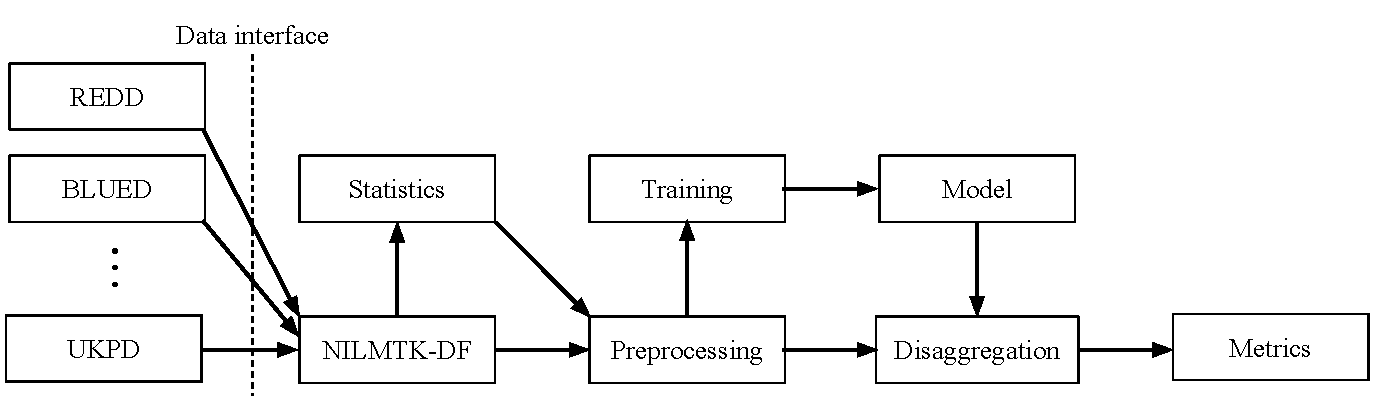
\includegraphics[scale=0.7]{figures/pipeline.pdf}
\caption{NILMTK pipeline. At each stage of the pipeline, results and data can be stored into or loaded from the disk.}
\label{fig:pipeline}
\end{figure*}

%\subsection{NILMTK pipeline}
%In this section we describe the implementation and design of NILMTK pipeline. 

%We now describe the implementation and design of each module of the NILMTK pipeline.

%\subsection{Dataset Importers}
\subsection{Data Format\bluecolor{maybe data interface?}}

\noindent
Motivated by our discussion on the wide differences between multiple data sets released in public domain in \secref{sec:related}, we propose NILMTK-DF, a common
data set format inspired by the REDD format~\cite{redd}, into which
existing data sets can be converted. NILMTK currently includes
importers for the following data sets: REDD, PECAN, HES, iAWE, AMPds
and UKPD. BLUED was excluded due to the lack of sub-metered appliance power data.Tracebase was not included due to the lack of information regarding which appliances were present in the same household.

After import, the data resides in our NILMTK-DF in-memory data structure, which is used throughout the NILMTK pipeline. Data can be saved or loaded from disk at multiple stages in the NILMTK processing pipeline to allow other tools to interact with NILMTK.  We provide two CSV flat file formats: a rich NILMTK-DF CSV format and a ``strict REDD" format which allows researchers to use their existing tools designed to process REDD data.  We also provide a more efficient binary format using the Hierarchical Data Format (HDF5).  In addition to storing electricity data, NILMTK-DF can also store relevant metadata and other sensor modalities such as gas, water, temperature, etc. It has been shown in the past that such additional sensor and metadata information may help enhance NILM prediction~\cite{schoofs_2010}. 

Another important feature of our format is standardisation of nomenclature.  Different data sets use different labels for the same class of appliance (e.g.\ REDD uses `refrigerator' whilst AMPds uses `FGE') and different names for the measured parameters.  When data is first imported into NILMTK, these diverse labels are converted to a standard vocabulary\bluecolor{Put a link where these are defined}.

%% Need to cut short
%\bluecolor{This again can potentially be represented as illustration better.}
In addition, NILMTK allows rich metadata to be associated with a building, appliance or meter.  For example, NILMTK can store the parameters measured by each meter (e.g.\ reactive power, real power), the geographical coordinates of each building (useful for exploring the relationship between appliance usage and weather), the mains wiring defining the meter hierarchy (useful if a single appliance is measured at the appliance, circuit and aggregate levels), whether a single meter measures multiple appliances, which appliances are not sub-metered and also whether a specific light is dimmable. A full description of NILMTK-DF is provided in \appref{app:appendix_data_format}.

%% Need to cut short- Maybe just a line or two
%% Should this even be included? it won't be ready for when the reviewers read the paper. Maybe it should be future work?
%Of course, we cannot hope to enumerate every possible appliance name and metadata attribute, hence we will use an instance of Semantic Mediawiki hosted at energy-disaggregation.org as the canonical source for the controlled vocabulary.  The wiki will make it easy for the community to add new appliance classes and metadata attributes.  Mediawiki has been used in other communities to create a collaborative controlled vocabulary; for example Open Street Map~\cite{haklay2008openstreetmap} use a wiki to maintain a list of `tags', and Semantic Mediawiki has been proposed as a mechanism for maintaining a controlled vocabulary for astronomical objects~\cite{chalmerscollaborative}.

%% This is interesting and should be there as a motivation!
Through such a combination of metadata and standard nomenclature, NILMTK further allows for analysis of data across multiple  data sets. For example, users can perform queries such as:
``what is the average energy consumption of refrigerators in the USA compared to the UK?"
%``how does the average energy consumption of fridges in the USA compare to fridges in the UK?"

\subsection{Data Set Statistics and Diagnostics}

\noindent
Due to a variety of challenges in collecting real world data, no data set is free of errors\bluecolor{most data sets contain gaps or missing values (I dont think its right to label them as errors) - or call something else but errors.}. Hence, researchers often need to spend a considerable amount of time exploring the detailed characteristics of each data set before proceeding with their research. One such common problem arises due to missing data.  Short gaps could be the result of 
%a random event causing 
the loss of a small number of radio transmissions from a wireless sensor. However, larger gaps are more likely to be caused by either a faulty or switched off sensor.
%(in which case the appliance state is unknown) or switched off (along with the attached appliance).  
To help diagnose these issues, NILMTK provides the following four functions\bluecolor{You may again refer to the specific section in your released documentation that talks about these 4 functions. 
At some point earlier - you may mention that detailed documentation is released and give the hyperlink. You may also mention that throughout the paper you will refer to specific sections of this documentation that provide further detail for the interested reader.}: a function to calculate the proportion of samples which are missing across an entire data set, %(with the option to either include or exclude large gaps)
a function to plot the dropout rate over time, a function to compute total sensor up-time and a function to compute contiguous sections of data. %\bluecolor{Again, too verbose description of functions to calculate statistics. Can be easily explained succinctly.}

NILMTK also provides functions for exploring appliance usage.  For example, the toolkit can calculate the distribution of appliance usage over repeating time periods, correlations between an appliance and weather conditions or across appliances, and the distributions of appliance power demands, on-durations and off-durations.  Furthermore, to explore the proportion of aggregate data which has been sufficiently sub-metered, NILMTK provides functions to calculate the proportion of time slices where a minimum percentage of the total energy has been sub-metered and also produces a list of the top-$k$ appliances across the time slices.

\subsection{Preprocessing}
\label{sec:preprocessing}

\noindent
The data sets described in \tabref{table:datasets} have been collected with a range of hardware, and under different settings.The sampling frequency of appliance monitors varies from 1 second to 2 minutes across the data sets.  NILMTK provide filters to down-sample data sets at a specified frequency. Further, these data sets have been collected from different countries, where the voltage fluctuations vary widely. Batra et al. showed voltage fluctuations from 180-250~V in the iAWE data set collected in India~\cite{iawe}, while the voltage variation in the SMART* data set is in the range 118-123~V. Hart et al.\ showed the need to take into account these voltage fluctuations as they can significantly impact power draw~\cite{hart_1992}. Therefore, as suggested by Hart, we also add a voltage normalisation function defined as follows: 
\begin{equation}
\textit{Power}_{\textit{normalised}} = 
\left(\frac{\textit{Voltage}_{\textit{nominal}}}{\textit{Voltage}_{\textit{observed}}}\right)^2 
\times \textit{Power}_{\textit{observed}}
\end{equation}
%Figure \redcolor{X} shows the power draw of an air conditioner, before and after voltage normalisation.

As explained in \secref{sec:training}, the memory required by some NILM algorithms is exponential in the number of appliances. Thus, when high number of appliances are considered, a single centralized model may not fit into memory, thus motivating the need for distributed algorithms. This necessitates the need to include top-$k$ appliances by their contribution which can be in terms of either energy or power.  We also created preprocessing functions for fixing other common issues with these datasets, such as 1) interpolating small periods of missing data when appliance sensors did not report readings; 2) filtering out implausible values (such as readings where observed voltage is more than twice the rated voltage) and 3) filtering out appliance data when mains data is missing.

\subsection{Training and Disaggregation}
\label{sec:training}
\noindent
NILMTK provides implementations of two common benchmark NILM algorithms: combinatorial optimisation (CO) and factorial hidden Markov model (FHMM). CO was proposed by Hart in his seminal work~\cite{hart_1992}, while techniques based on extensions of the FHMMs have been proposed recently\bluecolor{add some citations}. The aim of the inclusion of these algorithms is not to present state-of-the-art disaggregation results, but instead to enable new approaches to be compared to well-studied benchmark algorithms without requiring the reimplementation of such algorithms. We now briefly describe these two algorithms\bluecolor{may define NILM problem here}.
%It should be highlighted that the intended purpose of these algorithms is only to serve as benchmarks. We do not claim these to give the best results. We would encourage the community to get involved and submit their algorithms to NILMTK. 

\textbf{Combinatorial Optimisation:}
%\bluecolor{1-2 equations will be useful}
CO finds the \textit{optimal} combination of appliance states, which minimises the difference between the sum of the predicted appliance power and the observed aggregate power. 
\begin{equation}
\hat{x}^{(n)}_t=\operatorname*{arg min}_{\hat{x}^{(n)}_t}\left|\bar{y}_t-\sum\limits_{n=1}^{N}\hat{y}^{(n)}_t\right|
\end{equation}
Since each time slice is considered as a separate optimisation problem, each time slice is assumed to be independent.
%Its mathematical formulation is given as follows.
%CO assumes time samples to be independent and identically distributed (iid). 
CO resembles the subset sum problem and thus is NP-complete. The complexity of disaggregation for $T$ time slices is $O(TK^N)$, where $N$ is the number of appliances and $K$ is the number of states for each appliance. With the complexity of CO being exponential in the number of appliances, the approach is only computationally tractable when a small number of appliances are modelled.

\textbf{Factorial Hidden Markov Model:} The power demand of each appliance can be modelled as the observed value of a Gaussian Hidden Markov Model (HMM). The hidden component of these HMMs are the states of the appliances. Energy disaggregation involves jointly decoding the power draw of $n$ appliances and hence a factorial HMM~\cite{fhmm} is well suited. A FHMM can be represented by an equivalent HMM in which each state corresponds to a different combination of states of each appliance. The complexity of disaggregation for such a model is $O(TK^{2N})$, and as a result FHMMs scale even worse than CO. Such a FHMM model has three parameters: i) prior probability ($\pi$) containing $K^N$ entries, ii) transition matrix ($A$) containing $K^N~*K^N$ or $K^{2N}$ entries, and iii) emission matrix ($B$) containing $2K^N$ entries. From an implementation perspective, even storing (or computing) $A$ for 14 appliances with 2 states each needs 8 GB of RAM. Hence, we propose to validate FHMMs on preprocessed data where either top-$k$ appliances are considered, or appliances contributing less than a threshold are discarded.

For certain algorithms like FHMMs, modeling relationships amongst consecutive samples is necessary. Thus, NILMTK provides facilities for dividing data into train and test while still maintaining the notion of time.
\subsection{Model Import and Export}

%\redcolor{I think the argument here should be: benchmark algos require sub-metered data -> sub-metered data is not available in real deployments -> recent training methods have been proposed which do not require sub-metered data -> need an interface between training and disag to support different training methods}

\noindent
Recently, a lot of interest has arisen in deploying live NILM systems, as evidenced by the many startup companies (e.g.\ Energy Aware, PlotWatt, Bidgely, etc.) currently aiming to provide disaggregated consumption feedback to end consumers. Application of recent NILM algorithms proposed in academic research for live disaggregation is hindered by their primary suitability for offline statistical analysis of fixed data sets. Motivated by reducing the barrier from offline algorithms to those suitable for live deployments, we developed the Model module in NILMTK which encapsulates the results of the training module required by the disaggregation module. It is the responsibility of the model developer to create export and import functions to interface with a JSON file. NILMTK currently includes importers and exporters for both the FHMM and CO approaches. Further, in \secref{sec:use_case}, we show how if the rated power is known, we can avoid learning on sub-metered data. At the time of deployment, this learnt JSON model can be easily imported and used for disaggregation.

\subsection{Accuracy Metrics}

\noindent
As discussed in \secref{sec:related}, a range of accuracy metrics are required due to the diversity of application areas of energy disaggregation approaches. To satisfy this requirement, NILMTK provides a set of standard metrics. 
%This will allow researchers to evaluate different energy disaggregation algorithms using identical accuracy measures.
We now give a brief description of each metric along with its mathematical definition.\bluecolor{for each metric give relevant citations.}

%error energy
\textbf{Error in total energy assigned:} Represents the difference between the total energy assigned to appliance $n$ and the actual energy consumed by appliance $n$ over the entire data set.
\begin{equation}
%error^{(n)} = 
        \left | \sum_t y^{(n)}_t - \sum_t \hat{y}^{(n)}_t \right |
\end{equation}

%fraction energy assigned correctly
\textbf{Fraction of total energy assigned correctly:} Represents the overlap between the fraction of total energy assigned to each appliance and the actual fraction of total energy consumed by each appliance over the entire data set.
\begin{equation}
%fraction = 
        \sum_n \mathrm{min} \left ( 
        \frac{\sum_n y^{(n)}_t}{\sum_{n,t} y^{(n)}_t}, 
        \frac{\sum_n \hat{y}^{(n)}_t}{\sum_{n,t} \hat{y}^{(n)}_t} 
        \right )
\end{equation}

%mean normalised error power
\textbf{Normalised error in assigned power:} Represents the sum of the differences between the power assigned to appliance $n$ and the actual power of appliance $n$ in each time slice $t$, normalised by the total energy consumption of appliance $n$.
\begin{equation}
%error^{(n)} = 
        \frac
        { \sum_t {\left | y_t^{(n)} - \hat{y}_t^{(n)} \right |} }
        { \sum_t y_t^{(n)} }
\end{equation}

%rms error power
\textbf{RMS error in assigned power:} Represents the root mean square error between the power assigned to appliance $n$ and the actual power of appliance $n$ in each time slice $t$.
\begin{equation}
%error^{(n)} = 
\sqrt{ \frac{1}{T} \sum_t{ \left ( y_t - \hat{y}_t \right )^2 } }
\end{equation}

%confusion matrices
\textbf{Confusion matrix:} Represents the number of time slices in which each of an appliance's states were either confused with each other state or correctly classified.

%tp fp fn tn
\textbf{True positives, False positives, False negatives, True negatives:} Represents the number of time slices in which appliance $n$ was either correctly classified as being on~($\mathit{TP}$), classified as being on while it was actually off~($\mathit{FP}$), classified as off while is was actually on~($\mathit{FN}$), and correctly classified as being off~($\mathit{TN}$).
\begin{equation}
\mathit{TP}^{(n)} = 
\sum_{t}
\mathrm{AND} \left ( x^{(n)}_t = \mathit{on}, \hat{x}^{(n)}_t = \mathit{on} \right )
\end{equation}
\begin{equation}
\mathit{FP}^{(n)} = 
\sum_{t}
\mathrm{AND} \left ( x^{(n)}_t = \mathit{off}, \hat{x}^{(n)}_t = \mathit{on} \right )
\end{equation}
\begin{equation}
\mathit{FN}^{(n)} = 
\sum_{t}
\mathrm{AND} \left ( x^{(n)}_t = \mathit{on}, \hat{x}^{(n)}_t = \mathit{off} \right )
\end{equation}
\begin{equation}
\mathit{TN}^{(n)} = 
\sum_{t}
\mathrm{AND} \left ( x^{(n)}_t = \mathit{off}, \hat{x}^{(n)}_t = \mathit{off} \right )
\end{equation}

%tpr fpr
\textbf{True/False positive rate:} Represents the fraction of time slices in which appliance $n$ was correctly predicted to be on that it was actually on~($\mathit{TPR}$), and the fraction of time slices in which appliance $n$ was incorrectly predicted to be on that it was actually off~($\mathit{FPR}$).
\begin{equation}
\mathit{TPR}^{(n)} = \frac{\mathit{TP}}{\left ( \mathit{TP} + \mathit{FN} \right )}
\end{equation}
\begin{equation}
\mathit{FPR}^{(n)} = \frac{\mathit{FP}}{\left ( \mathit{FP} + \mathit{TN} \right )}
\end{equation}

%precision recall
\textbf{Precision, Recall:} Represents the fraction of time slices in which appliance $n$ was correctly predicted to be on that it was actually off~(Precision), and the fraction of time slices in which appliance $n$ was correctly predicted to be on that it was actually on~(Recall)
\begin{equation}
\mathit{Precision}^{(n)} = \frac{\mathit{TP}}{\left ( \mathit{TP} + \mathit{FP} \right )}
\end{equation}
\begin{equation}
\mathit{Recall}^{(n)} = \frac{\mathit{TP}}{\left ( \mathit{TP} + \mathit{FN} \right )}
\end{equation}

%f score
\textbf{F-score:} Represents the harmonic mean between precision and recall.
\begin{equation}
\mathit{F\text{-}score}^{(n)} = \frac
            {2 . \mathit{Precision} . \mathit{Recall}}
            {\mathit{Precision} + \mathit{Recall}}
\end{equation}

%hamming loss
\textbf{Hamming loss:} Represents the total information lost when appliances are incorrectly classified over the data set.
\begin{equation}
\mathit{HammingLoss} = 
        \frac{1}{T} \sum_{t}
        \frac{1}{N} \sum_{n}
        \mathrm{XOR} \left ( x^{(n)}_t, \hat{x}^{(n)}_t \right )
\end{equation}



\noindent
In \appref{app:appendix_pipeline} we summarise the NILMTK pipeline with a code snippet to illustrate the ease by which data sets can be imported and preprocessed, algorithms can be trained and used to disaggregate a household's energy usage, and accuracy metrics can be employed to evaluate disaggregation accuracy.


\section{Evaluation}
\label{evaluation}

\noindent
We now demonstrate several examples of rich analysis supported by NILMTK. First, we show how existing data sets can be processed to produce representations of the quality of data and the also to provide details regarding the appliances present in the data set. Second, we give some examples of the effect of voltage normalisation on the power demand of individual appliances, and discuss how this might affect the performance of a disaggregation algorithm. Third, we present summary performance results of the two benchmark algorithms included in NILMTK across four data sets using a number of accuracy metrics. Fourth, we present detailed results of these algorithms for a single data set, and discuss each algorithm's performance for different appliances.

\subsection{Summary of datasets}
\bluecolor{There are too many plots in this section. If you need space this is the candidate section where you may delete. Ex. Figure 2 and Figure 5 can potentially go away.}
\noindent
\tabref{table:dataset_results} shows a selection of statistics
across multiple public datasets.  These statistics were calculated by
the stats functions in NILMTK.  

Figure~\ref{fig:lost_samples} shows the distribution of lost samples for REDD house 1.  From this we can see that the two mains channels have four large gaps, but otherwise the mains have a dropout rate near to zero. The sub-metered channels have only one large gap but, ignoring this gap, the sub-metered channels have a constant dropout rate of about \redcolor{20\%}.\bluecolor{Did authors give any intuition for why there is such a constant dropout rate observed}

\begin{figure}[!t]
  \centering
  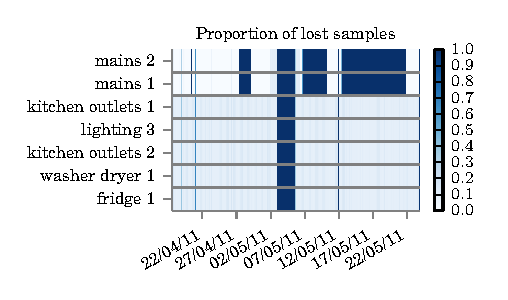
\includegraphics[width=\columnwidth]{figures/lost_samples.pdf} 
  \caption{Lost samples from REDD house 1.  Light blue indicates a low
    dropout rate; dark blue indicates a high dropout rate.  The figure
    only shows a subset of the submetered channels.\bluecolor{The figure is not very clear. What is the time window that you took when calculating the drop-out rate?}}
  \label{fig:lost_samples} 
\end{figure}

\begin{table*}[]
  \centering
\begin{tabular}{cccccc}
\hline
\textbf{Data set} & \textbf{\specialcell[h]{Number of\\appliances}} & \textbf{\specialcell[h]{Percentage\\energy\\sub-metered}} & \textbf{\specialcell[h]{Percentage\\missing samples\\(ignoring gaps)}} & \textbf{\specialcell[h]{Mains up-time\\per building\\(days)}} & \textbf{\specialcell[h]{Percentage\\up-time}} \\
\hline
REDD & 9, 16, 23 &58, 71, 89 & 0, 10, 16 &4, 18, 19 & 8, 40, 79 \\
Pecan Street &13, 14, 22 & 75, 87, 150 & 0, 0, 0 &7, 7, 7 & 100, 100, 100 \\
AMPds&20 &97 & 0 &364 & 100 \\
iAWE &10 &48 & 8 & 47 &93 \\
UKPD & 4, 12, 49 &19, 48, 82 &0, 7, 22 & 36, 102, 404 & 73, 84, 100 \\
\hline
\end{tabular}
  \caption{Summary of data set results calculated by the statistics
    functions in NILMTK.  Each cell represents the range of values
    across all buildings per data set.  The three
    numbers per cell are the minimum, median and maximum values. AMPds
    and iAWE each contain just a single building, hence these rows
    have a single number per cell.  Large gaps in each channel were
    removed prior to calculating ``percentage energy sub-metered'',
    ``percentage missing samples'' and ``mains up-time''.  (By ``gap''
    we mean any period between two samples longer than 20 $\times$ the
    sample period).  iAWE data was cropped to 2013/6/11 to
    2013/7/31. \bluecolor{Refer to the page on your public documentation which explains what each of these statistics really mean. Its not very obvious to me what does percentage up-time mean.} \redcolor{todo: investigate which chans are causing two
      Pecan homes to have \% energy submetered above 100\%, do
      Smart*}}
  \label{table:dataset_results}
\end{table*}


\subsubsection{Appliance power profiles}

\noindent
Each appliance consumes a range of
powers\bluecolor{I dont know if this statement is true. An appliance may be consuming constant power but the variation could be due to voltage variation or noise in power line. You may just delete this sentence as well.}. Figure~\ref{fig:power_histograms} displays histograms of the
distribution of powers used by a selection of appliances.  Appliances
like toasters and kettles tend to have only two possible power states:
on and off.  This simplicity makes them amenable to be modelled by,
for example, Markov chains with only two states per chain.  Appliances
like washing machines, hoovers, dimmable lights and computers often
have more than two power states.

The proportion of energy use per appliance varies from country to
country. For example, the building recorded in India for the iAWE
dataset has two air conditioning units; whilst none of the buildings
in UKPD have any air conditioning unit.  The differences in appliance
energy use by country are illustrated in Figure~\ref{fig:pie}.

\begin{figure*}
  \centering
  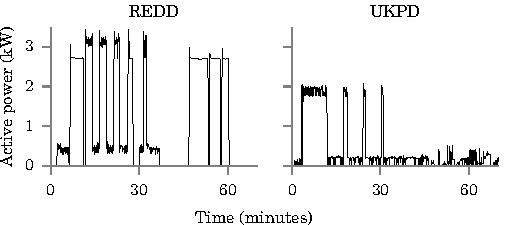
\includegraphics{figures/wm.pdf}
  \caption{Comparing American and UK washing machines.\bluecolor{not referred anywhere--maybe even in single column}}
  \label{fig:wm}
\end{figure*} 

\begin{figure*}
 \centering
 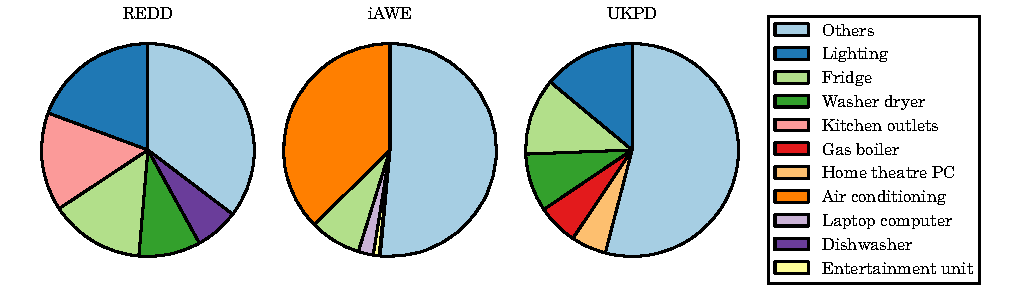
\includegraphics{figures/top_k_appliances_pie.pdf}
 \caption{Top 5 appliances in terms of the proportion of the total
   energy used in building 1 in each of REDD (USA), iAWE (India) and
   UKPD (UK). Energy use of multiple appliances in the same category is added.}
 \label{fig:pie}
\end{figure*}

\subsubsection{Learning usage patterns}

\noindent
Modern automatic speech-to-text systems not only learn to map phonemes
to characters but also learn which phonemes tend to appear together
and which words tend to appear together.  In a similar fashion, a
disaggregation system might learn not just to recognise the appearance
of individual appliances in an aggregate signal but might also learn
when particular appliances are usually active each day (e.g. the TV is
usually on in the evening), correlations between appliances (e.g. the
office LCD screen is on when the office PC is on) and correlations
between appliances and additional information such as weather data
from the local meteorological office (e.g. less sunshine implies more
usage of electric lights).

One probabilistic learning framework capable of capturing this
information is the Conditional Factorial Hidden Markov Model (CFHMM)
proposed by Kim et. al.~\cite{kim_2011}. They also presented
several examples of such patterns.  Prior knowledge from
public datasets could be used to create general probability
distributions for each appliance class and these distributions could
then be refined by the disaggregation system for each house.

In the following sections, we present patterns of appliance usage per
day and per week; correlations between appliance usage and weather
variables; and histograms of appliance on-durations. 

\subsubsection{Usage histograms}

\begin{figure}[!t]
  \centering
  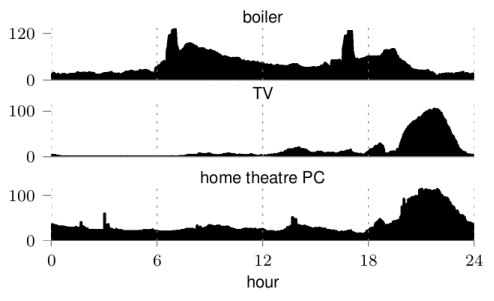
\includegraphics[width=\columnwidth]{figures/daily_usage_histograms2.pdf}
  \caption{Daily appliance usage histograms for a selection of
    appliances for data from UKPD Building 1 (bin width = 1 minute).}
  \label{fig:daily_usage_histograms}
\end{figure} 

\noindent
\bluecolor{You may make this subsection of the previous section. Otherwise previous section as a standalong subsection does not look good. Or just give these labels without assigning them sub-sub-sub sections.}
Histograms showing usage patterns for a selection of appliances over
an average day are shown in Figure~\ref{fig:daily_usage_histograms} from which strong similarities between groups of appliances can be seen.  \bluecolor{Try to be consistent with what you write and what you show. Currently your examples are not what is shown in the figure.}For
example, the usage pattern of the TV and ``amp livingroom'' are very
similar because the amp is used to play the TV's audio but the amp is
sometimes on without the TV.  Similarly, the kitchen lights, kettle
and toaster show similar usage patterns.

To produce these usage histograms, we applied a manually-configured
power threshold to each appliance.  We were interested in user
behaviour but the data set was recorded using UTC timestamps and the
data set spans a daylight saving transition from GMT to BST.  As such,
all times were converted to local time to produce these histograms.
The use of local time has produced one artefact: the small ``bump''
towards the right of the solar thermal pump histogram\bluecolor{where is it?} in
Figure~\ref{fig:daily_usage_histograms} (the earth's rotation does not
alter in response to day light saving transitions!).

\subsubsection{Correlations with weather}

\noindent
We expect the usage of some appliances to be correlated with some
weather variables.  Previous studies have demonstrated correlations
between temperature and heating/cooling demand in
Australia~\cite{RicharddeDear2002} and between temperature and total
household electricity usage in America~\cite{Kavousian2013a}.  We
wanted to search for similar correlations.

If robust correlations can be demonstrated then a disaggregation
system could learn correlations between weather variables and
appliance usage in order to refine its appliance usage estimates. \redcolor{cite Kolter's December 2013 paper}
Weather data are relatively easy to acquire programmatically: for
example, the UK Metoffice provides free access to live weather data
via their DataPoint API.

Figure~\ref{fig:weather_correlations} shows correlations between
boiler usage and maximum temperature.  The correlation between
external maximum temperature and boiler usage is strong ($R^2=0.73$); and it is
noteworthy that the X-axis intercept ($\approx19\,^{\circ}\mathrm{C}$)
is approximately the set point for the boiler thermostat, as one might
expect.  Lighting circuit usage also correlates with solar radiation
(not shown) although there is considerable variation in lighting usage
which is not explained by solar radiation.

\begin{figure}[!t]
  \centering
  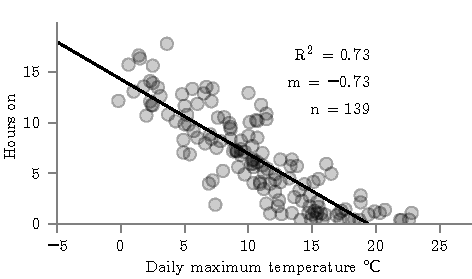
\includegraphics[width=\columnwidth]{figures/weather_correlations2.pdf} 
  \caption{Linear regression showing correlation between gas boiler
    usage and external temperature. $R^2$ denotes the coefficient of
    determination, $m$ is the gradient of the regression line and $n$
    is the number of data-points used in the regression.  Each
    data-point represents one day.  Appliance
    data from UKPD building 1.  Historical daily averages from
    Heathrow weather station (20 miles west of UKPD building 1) were
    obtained from the UK Met Office under their Educational program.
    Days when the appliance usage was zero were ignored because
    we assume that the house was unoccupied on these days.\bluecolor{make figure x and ylabels c; reduce caption}}
  \label{fig:weather_correlations} 
\end{figure}

%\subsection{The curious case of voltage normalisation}
\subsection{Voltage normalisation} % more formal

\noindent
Mains voltage usually fluctuates around the nominal value. In the UK, for example, it is nominally 230\;V but is allowed to vary by
$-6\%,\;{+10}\%$.  This variation in voltage can produce a variation in power consumption of -12\% to +20\% \bluecolor{confirm this once}in linear loads like resistive heaters because $P=I \times V$ and because current changes with voltage
for resistive loads according to Ohm's law ($I=\sfrac{V}{R}$).
These abrupt changes in reported power due to voltage fluctuations can be
problematic for disaggregation algorithms.  To mitigate this effect, we can normalise the power consumption, as outlined in Section \ref{sec:preprocessing}.

Figure~\ref{fig:power_histograms} shows
histograms for both the normalised and un-normalised appliance power
consumption. Normalisation produces a noticeably tighter power
distribution for linear resistive devices such as the toaster but has
little effect on constant power appliances such as TVs\bluecolor{TV is not shown in Figure 7. Give examples of something that you show or vice versa.} whose power consumption does
not vary significantly as voltage varies because their power supplies are designed to draw the same power across the permissible voltage range.

\begin{figure*}[!t]
  \centering
  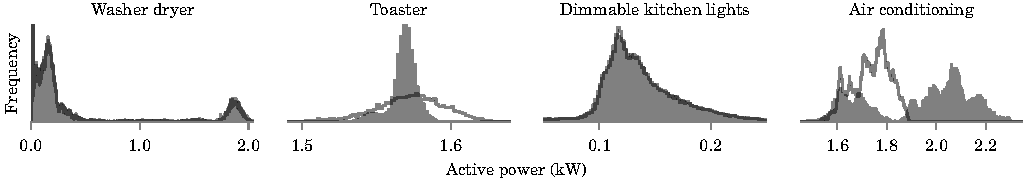
\includegraphics{figures/power_histograms.pdf} 
  \caption{Histograms of power consumption. The filled grey plots show
    histograms of ``normalised power''.  The thin, grey,
    semi-transparent lines drawn over the filled plots show histograms
    of un-normalised power.  The ``air conditioning'' data is from
    iAWE, the ``washer dryer'' and ``toaster'' are from UKPD building 1. \bluecolor{Explain why AC is not good..}}
  \label{fig:power_histograms} 
\end{figure*}

\subsection{Disaggregation across datasets}

\noindent
We now compare the disaggregation results across the first home of each of the following 6 datasets: AMPds, PECAN, iAWE, Smart*, UKPD and REDD. Since all the datasets were collected for different durations, we used fist half the samples for training and remaining half for testing across all the datasets. Further, we preprocessed datasets such as REDD, UKPD and iAWE to 1 minute frequency using the downsampling filter to account for different aggregate and mains data sampling frequencies and compensating for intermittent lost data packets. 
As highlighted above, REDD and iAWE also have significant proportion of missing data, which were appropriately preprocessed. AMPds and PECAN data did not require any preprocessing. Apart from REDD, Smart*, UKPD and iAWE, the remaining datasets were processed at the frequency at which they were made available (i.e.\ PECAN - 1 minute, AMPds - 1 minute). Since both CO and FHMM have exponential computational complexity in the number of appliances, we consider only those appliances whose contribution was greater than 5\%. Across all the datasets, the appliances which contribute more than 5\% of the aggregate include HVAC appliances such as the air conditioner and thermostats, and appliances which are used throughout the day such as the refrigerator. We compare the disaggregation performance of CO and FHMM across the following three metrics: 1) Fraction of total energy assigned correctly (FTE), 2) Normalised error in assigned power (NEP), 3) F-score. These three metrics and their variations have been used most often in prior NILM work. %The results are summarised in \tabref{table:disaggregation}.
A lower NEP indicates better performance, while in contrast a higher F-score and FTE indicate better disaggregation accuracy. The evaluation was performed on a laptop having 2.3 GHz i7 processor and 8 GB RAM running Linux.

%Table~\tabref{table:disaggregation} summarises the results of the two algorithms across the four data sets. It can be seen that across all the metrics, CO performance is similar to FHMM performance in iAWE and PECAN. In both the used homes from these two datasets, space heating contributes very significantly (about 60\% for a single air conditioner which has a power draw of ~2700 W in the PECAN home and about \redcolor{40\%} across two air conditioner having a power draw of ~1700W and ~1200W respectively. These appliances are easier to disaggregate owing to their huge power demand in comparison to appliances such as electronics and lighting. However, in the first homes used from REDD and AMPds dataset, the power consumption is spread across a lot more number of appliances. A significant number of appliances (14 in AMPds home and 13 in REDD) each contribute less than 5\% of the total load. Under such circumstances, it can be observed that FHMM performance is superior to CO performance across the three metrics. This confirms the theoretical foundations propounded by Hart et al.\cite{hart_1992}; that CO is highly sensitive to small variations in the aggregate load. In contrast, FHMM overcomes these by considering an associated transition probability between states. We further discuss 

\tabref{table:disaggregation} summarises the results of the two algorithms across the four data sets. It can be observed that FHMM performance is superior to CO performance across the three metrics for both REDD and AMPds. This confirms the theoretical foundations proposed by Hart~\cite{hart_1992}; that CO is highly sensitive to small variations in the aggregate load. FHMM approach overcomes these shortcoming by considering an associated transition probability between the different states of an appliance. However, it can be seen that CO performance is similar to FHMM performance in iAWE, PECAN, Smart* and UKPD across all metrics. This is likely due to the fact that in selected homes from these datasets, very few appliances contribute more than 5\% of the aggregate. For instance, space heating contributes very significantly (about 60\% for a single air conditioner which has a power draw of ~2700 W in the PECAN home and about 35\% across two air conditioner having a power draw of ~1800W and ~1600W respectively). As a result, these appliances are easier to disaggregate by both algorithms, owing to their relatively high power demand in comparison to appliances such as electronics and lighting. Whereas, in the UKPD home, washing machine was one of the appliance contributing more than 5\% of the aggregate, which brought down overall metrics across both approaches. 
%However, in the first homes used from REDD and AMPds dataset, the power consumption is spread across a lot more number of appliances. A significant number of appliances (14 in AMPds home and 13 in REDD) each contribute less than 5\% of the total load. Under such circumstances,  

Another important aspect to consider is the time required for testing and training. These timings confirm the fact that CO is exponentially quicker than FHMM. This raises an interesting insight: In homes such as the ones used from PECAN and iAWE in the above analysis, it may be beneficial to use CO over a FHMM owing to the less amount of time required for training and testing, even though FHMMs are in general considered to be more powerful.

\begin{table*}
\centering
\begin{tabular}{ccccccccccc}
\hline\textbf{Dataset} & \multicolumn{2}{c}{\textbf{Train time (s)}}& \multicolumn{2}{c}{\textbf{Disaggregate time (s)}} &\multicolumn{2}{c}{\textbf{NEP}}    & \multicolumn{2}{c}{\textbf{FTE}} &\multicolumn{2}{c}{\textbf{F-score}} \\ 
~ &\textbf{CO} & \textbf{FHMM} &\textbf{CO} & \textbf{FHMM} &\textbf{CO} & \textbf{FHMM} &\textbf{CO} & \textbf{FHMM}&\textbf{CO} & \textbf{FHMM} \\ \hline 
REDD &3.67 &22.81 &0.14 &1.21 &1.61 &1.35 &0.77 &0.83 &0.31 &0.31\\ 
SMART* &1.51 &1.66 &0.03 &0.09 &0.75 &0.70 &0.89 &0.93 &0.80 &0.79\\ 
PECAN &1.72 &2.83 &0.02 &0.12 &0.68 &0.75 &0.99 &0.87 &0.77 &0.77\\ 
AMPds &5.92 &298.49 &3.08 &22.58 &2.23 &0.96 &0.44 &0.84 &0.55 &0.71\\ 
iAWE &1.68 &8.90 &0.07 &0.38 &0.91 &0.91 &0.89 &0.89 &0.73 &0.73\\ 
UKPD &1.06 &11.42 &0.10 &0.52 &3.66 &3.67 &0.81 &0.80 &0.38 &0.38\\
\hline
\end{tabular}
\caption{Comparison of CO and FHMM across multiple datasets\bluecolor{Can you also mention number and possibly name as well of appliances disaggregated for each dataset?}}
\label{table:disaggregation}
\end{table*}

\subsection{Detailed disaggregation results	}


\begin{table}
    \begin{tabular}{ccccc}
    \hline \textbf{Appliance} & \multicolumn{2}{c}{\textbf{NEP}} & \multicolumn{2}{c}{\textbf{F-score}}\\
    ~                  & \textbf{CO}    & \textbf{FHMM}  & \textbf{CO}      & \textbf{FHMM} \\ \hline
    Air conditioner 1  & 0.3   & 0.3   & 0.9     & 0.9  \\
    Air conditioner 2  & 1.0   & 1.0   & 0.7     & 0.7  \\
    Entertainment unit & 4.2   & 4.1   & 0.3     & 0.3  \\
    Fridge             & 0.5   & 0.5   & 0.8     & 0.8  \\
    Laptop computer    & 1.7   & 1.8   & 0.3     & 0.2  \\
    Washing machine    & 130.1 & 125.1 & 0.0     & 0.0  \\
    \hline \end{tabular}
    \caption{Comparison of CO and FHMM across different appliances in iAWE dataset}
\label{table:disaggregation_iawe}
\end{table}


\begin{figure}
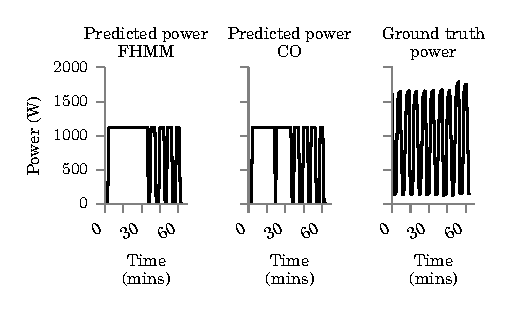
\includegraphics{figures/ac_2.pdf} 
\caption{Comparison of predicted power (CO and FHMM) with ground truth for air conditioner 2 in the iAWE dataset}
\label{fig:ac_disaggregation} 
\end{figure}

\noindent
Having compared disaggregation results across different datasets, we now do a detailed discussion of disaggregation results across different appliances for a single home in the iAWE dataset in \tabref{table:disaggregation_iawe}. As before, we model all appliances using 2 states. In order to show the disagregation performance across appliances, we choose the top 6 appliances by their energy consumption. We observe that CO and FHMM report similar performance across all the appliances. We observe that across both metrics results for appliances such as washing machine and SMPS based appliances such as laptop and entertainment unit(television) are much worse when compared to HVAC loads like air conditioners. It is well known in prior literature that appliances such as washing machines are hard to model~\cite{barker_2013}.

We observe that the performance accuracy of air conditioner 2 is much worse than air conditioner 1. This is due to the fact that during the instrumentation, air conditioner 2 was operated at a set temperature of $26\,^{\circ}\mathrm{C}$. With external temperature roughly $5-10\,^{\circ}\mathrm{C}$ below this set temperature, this air conditioner reached the set temperature quickly and turned off the compressor while still running the fan. However, air conditioner 1 was operated at operated at $16\,^{\circ}\mathrm{C}$ and mostly had the compressor on. Thus, air conditioner 2 spent much more time in this intermediate state (compressor off, fan on) in comparison to air conditioner 1. \figref{fig:ac_disaggregation} shows how both FHMM and CO are able to detect on and off events of air conditioner 2. Since air conditioner 2 spent considerable amount of time in the intermediate state, the learnt 2 state model is less appropriate in comparison to the 2 state model used for air conditioner 1. This can be further seen in \figref{fig:ac_disaggregation}, where we observe that both FHMM and CO learn a much lesser power level of around 1100 W, in comparison to the rated power of around 1600 W.\bluecolor{Why are you able to detect cycles more accurately after 30 minutes and not before 30 minutes?} We believe that this can be corrected by choosing a more appropriate 3 state model for this air conditioner, which comes at a cost of increased training and disaggregation computational and memory requirements. The air conditioner set temperature details quoted above were provided by the iAWE authors as a part of appliance metadata in their dataset release.



%\subsection{Effect of sampling rate}

\section{Case Studies}
\label{sec:use_case}
We now consider two deployment scenarios where NILMTK is being used to perform disaggregation. Firstly, we consider the faculty housing deployment at IIIT Delhi~\cite{batra_2012}. 26 apartments have been instrumented individually with smart meters. Data from these homes is being aggregated into a sMAP~\cite{smap} server instance residing inside IIIT Delhi. Aggregate home data from sMAP is pulled via HTTP request and is fed into NILMTK via a converter. The aim of this experiment was to understand if rated power can suffice for disaggregating large HVAC based loads such as air conditioner and room heaters. Thus, we fed the rated power of different appliances into CO JSON model and disaggregated on the aggregate data. We found that this approach worked sufficiently well in disaggregating HVAC based loads\bluecolor{may include a plot or remove the section completely}. The second user study was a single home deployment in \redcolor{Delhi/London} where the data from the smart meter was collected using a low power \redcolor{RPi/Intel Atom}.

\section{Conclusions and future work}
\label{sec:conclusions}

\noindent
In this paper, we proposed NILMTK; an open source toolkit designed to allow empirical comparisons to be made between existing energy disaggregation algorithms. The toolkit defines a common data format, NILMTK-DF, provides parsers from \redcolor{X} publicly available data sets to NILMTK-DF, and provides data set statistics and preprocessing functions to identify and mitigate common problems with NILM data sets. In addition, the toolkit includes implementations of two benchmark disaggregation algorithms based on combinatorial optimisation and the factorial hidden Markov model. Furthermore, NILMTK includes implementations of a set of performance metrics which will enable future research to directly compare disaggregation approaches through a common set of accuracy measures.

\redcolor{Paragraph on benefits of benchmark algo evaluations.}

Future work will focus upon the addition of recently proposed disaggregation algorithms. For instance, both benchmark implementations included in NILMTK are well studied algorithms which require sub-metered appliance data from each household for a supervised training phase, while algorithms proposed in more recent research~\cite{kim_2011,parson_2012} only require aggregate data for an unsupervised training phase.  These algorithms are computationally expensive so a GPU implementation may be explored.

An additional direction for future work would be the inclusion of a household simulator within NILMTK. Since all data sets represent a limited number of households, and it is currently impossible to test how a disaggregation algorithm might perform in a household other than those present in existing data sets. However, a simulator would overcome this problem by generating data for new households by either combining appliance data from multiple households or simulating appliances using detailed appliance models.

%\section{Acknowledgements}

%\noindent
%Nipun Batra would like to thank TCS Research and Development for supporting him through a PhD fellowship and EMC, India for their support. The authors would also like to thank the Department of Electronic and Information Technology (DEITy), Government of India for funding the project (Grant Number DeitY/R\&D/ITEA/4(2)/2012). Jack Kelly would like to thank the EPSRC for his Doctoral Training Account and Intel for their PhD Fellowship grant. 

\bibliographystyle{abbrv}
{\scriptsize
\bibliography{reference}}

\newpage
\appendix
\section{NILMTK-DF}
\label{app:appendix_data_format}
We now provide the details of NILMTK-DF. NILMTK-DF follows a hierarchical structure which models the physical hierarchies. 

\begin{figure}
\centering 
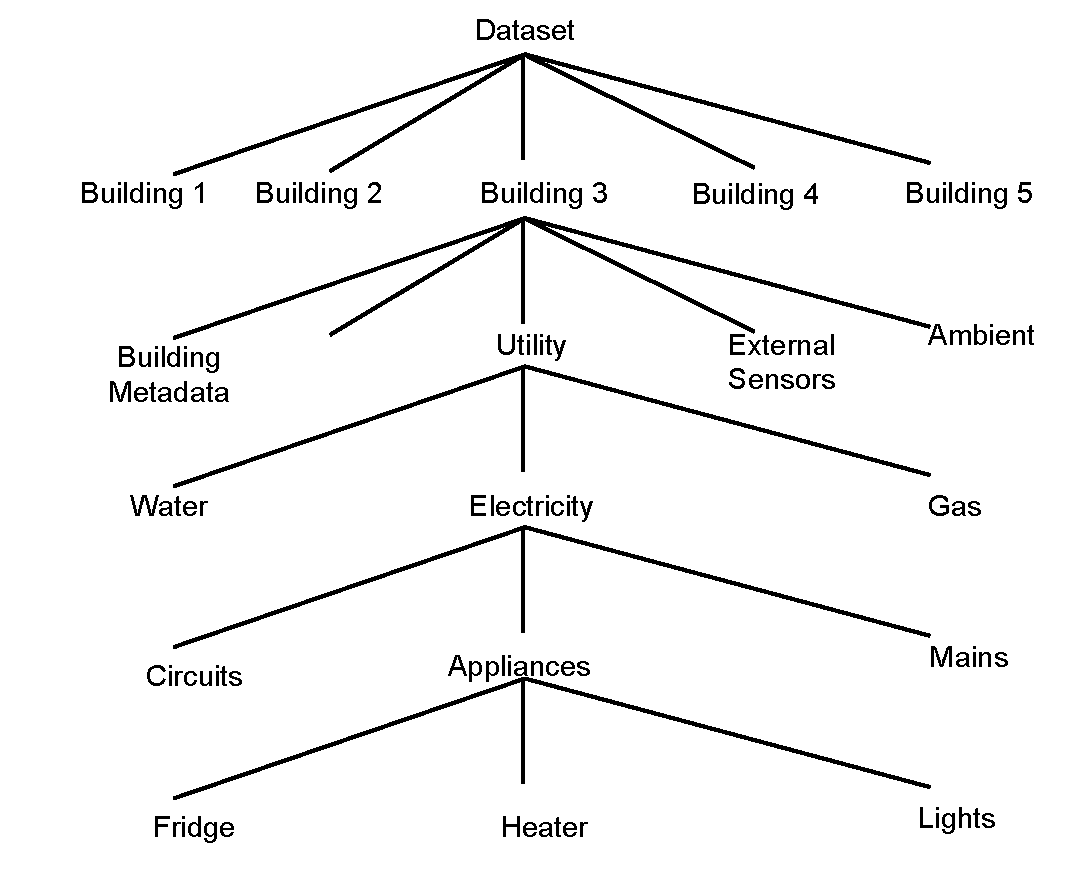
\includegraphics[scale=0.5]{figures/data_format.pdf}
\caption{NILMTK-DF format hierarchy}
\label{fig:nilmtk-format}
\end{figure}

\section{Sample code for NILMTK pipeline}
\label{app:appendix_pipeline}
We now illustrate the NILMTK pipeline via a minimal code example.

\begin{verbatim}
dataset = DataSet()

#Load the dataset
dataset.load_hdf5(DATASET_PATH)

#Load first building
building = dataset.buildings[1]

#Remove records where voltage>260 or voltage<160
building = filter_out_implausible_values(
    building, Measurement(`voltage', `'), 160, 260)
    
#Downsample to 1 minute
building = downsample(building, rule='1T')

# Choosing feature for disaggregation
DISAGG_FEATURE = Measurement(`power', `active')

# Dividing the data into train and test
train, test = train_test_split(building)

# Train on DISAGG_FEATURES using FHMM
disaggregator = FHMM()
disaggregator.train(train, 
            disagg_features=[DISAGG_FEATURE])
            
# Disaggregate
disaggregator.disaggregate(test)

# F1 score metric
f1_score = f1(disaggregator.predictions, 
            test)
\end{verbatim}

\section{Adding a new NILM algorithm}
Every algorithm needs to define the following four functions:
\begin{itemize}
\item train: The parameters of this function are the `building',
The parameters are inspired from R style formulas.
\item disaggregate
\item import model: 
\item export model:
\end{itemize}

%% \section{Appendix2}
%% This section includes content which we currently do not propose to include in the E-Energy paper but which may be included in an extended version of the paper on arXiv.  Or, if our supervisors like any of this content, then we will include it in the main paper.

%% \subsection{Summary of datasets}

%% \subsubsection{Usage histograms}

%% Usage patterns over an average week for the office LCD screen and
%% hoover are shown in figure~\ref{fig:weekly_usage_histograms}.  The
%% office LCD screen is used more frequently on weekdays than on
%% weekends; the inverse is true for the hoover.

%% \begin{figure}[!t]
%%   \centering
%%   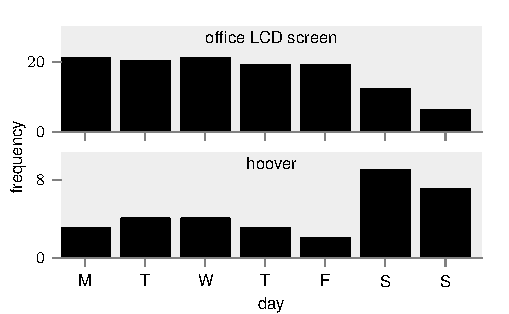
\includegraphics[width=\columnwidth]{figures/weekly_usage_histograms.pdf}
%%   \caption{Weekly appliance usage histograms for the office LCD screen
%%     (top panel) and hoover (bottom panel).  Data from UKPD building 1.}
%%   \label{fig:weekly_usage_histograms}
%% \end{figure}

%% Histograms of on-durations are displayed in
%% figure~\ref{fig:on_durations}. As identified by \cite{kim_2011}, the
%% gamma distribution would be a better fit for several appliance
%% on-durations than the exponential distribution.

%% \begin{figure*}[!t]
%%   \centering
%%   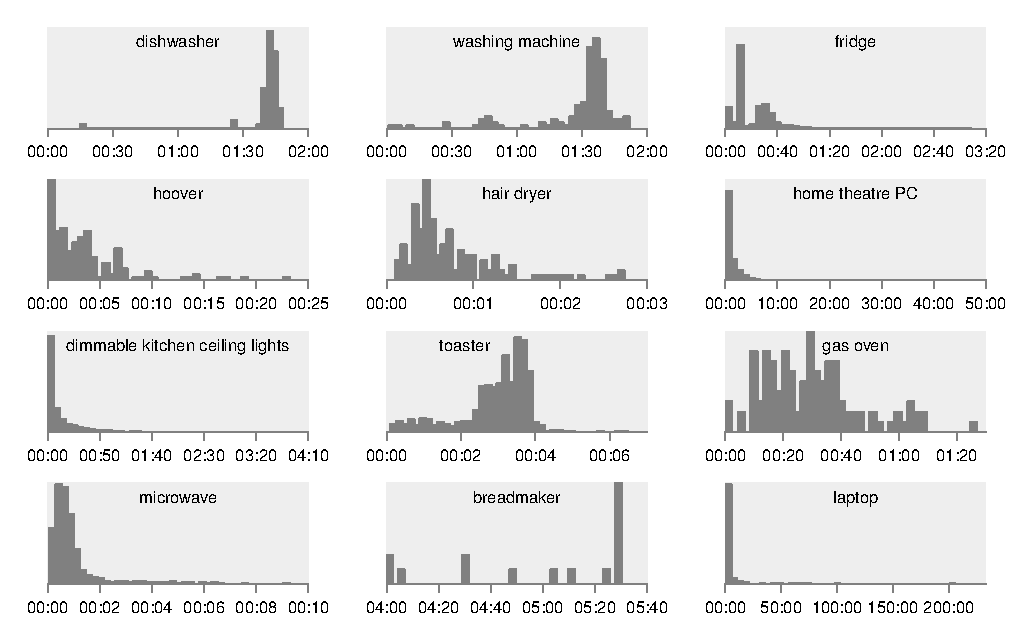
\includegraphics{figures/on_durations.pdf}
%%   \caption{On-durations for a selection of appliances.  The horizontal
%%     axis displays time formatted as ``hours:minutes''.  Outliers have
%%     not been removed.  The laptop was on for over 200 hours (8 days)
%%     while it was being used to collect data.  The home theatre PC was
%%     on for over 40 hours while it was re-installing its operating
%%     system.  Data from UKPD building 1.}
%%   \label{fig:on_durations}
%% \end{figure*}

%% \subsubsection{Correlations with weather}

%% An example of seasonal variation in boiler usage is shown in
%% figure~\ref{fig:seasonal_variation}.  During February, when the
%% weather is relatively cold in the UK, the boiler is primarily used to
%% heat to the radiators for the majority of the day.  In May, when the
%% weather is warmer, the space heating requirement drops away and the
%% twice-daily hot water heating program dominates the usage histogram.

%% \begin{figure}[!t]
%%   \centering
%%   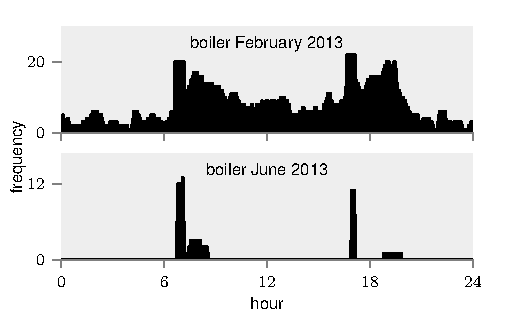
\includegraphics[width=\columnwidth]{figures/seasonal_variation.pdf}
%%   \caption{Seasonal variation in boiler usage.  In June (bottom panel),
%%     the boiler usage histogram is dominated by the hot water program
%%     which runs twice a day.  In February (top panel), considerably
%%     more energy is used on space heating than on hot water heating.   Data from UKPD building 1.}
%%   \label{fig:seasonal_variation}
%% \end{figure}

\end{document}
